\documentclass[aspectratio=169,11pt]{beamer}
\usetheme{metropolis}

\usepackage{listings}
\usepackage{listingsutf8}
\usepackage{fontspec}
\usepackage{textcomp}
\usepackage{graphicx}
\usepackage{tikz}
\usetikzlibrary{calc,arrows.meta,positioning}

% -- Colors ---------------------------------------------------------------
\definecolor{primary}{RGB}{0,102,204}
\definecolor{darktext}{RGB}{44,62,80}
\definecolor{codebg}{RGB}{245,245,245}
\definecolor{goblue}{RGB}{0,125,156}
\definecolor{removed}{RGB}{200,50,50}
\definecolor{added}{RGB}{40,160,60}
\definecolor{muted}{RGB}{130,130,130}
\definecolor{accent}{RGB}{230,126,34}
\definecolor{darkbg}{RGB}{35,35,45}
\definecolor{slidebg}{RGB}{250,250,252}

% -- Theme tweaks ----------------------------------------------------------
\setbeamercolor{frametitle}{bg=darkbg,fg=white}
\setbeamercolor{progress bar}{fg=primary}
\setbeamercolor{title separator}{fg=primary}
\setbeamercolor{alerted text}{fg=accent}
\setbeamercolor{normal text}{fg=darktext}
\setbeamercolor{background canvas}{bg=slidebg}

\setbeamerfont{title}{size=\large,series=\bfseries}
\setbeamerfont{subtitle}{size=\small}
\setbeamerfont{frametitle}{size=\large,series=\bfseries}
\setbeamerfont{section title}{size=\Large,series=\bfseries}

% -- Listings config -------------------------------------------------------
\lstdefinelanguage{Go}{
  keywords={package,import,func,return,var,type,struct,interface,if,else,for,range,switch,case,default,defer,go,chan,map,select,break,continue,fallthrough,const,nil,true,false,error,string,int,int64,float64,bool,byte,context,Context},
  keywordstyle=\bfseries\color{goblue},
  ndkeywords={http,slog,sync,fmt,errors,time,json,atomic},
  ndkeywordstyle=\color{primary},
  sensitive=true,
  comment=[l]{//},
  morecomment=[s]{/*}{*/},
  commentstyle=\itshape\color{muted},
  stringstyle=\color{accent},
  morestring=[b]",
  morestring=[b]`,
}
\lstset{
  language=Go,
  basicstyle=\ttfamily\tiny,
  backgroundcolor=\color{codebg},
  frame=single,
  rulecolor=\color{muted!40},
  framesep=3pt,
  xleftmargin=4pt,
  xrightmargin=4pt,
  breaklines=true,
  showstringspaces=false,
  tabsize=8,
  columns=fullflexible,
  keepspaces=true,
  aboveskip=4pt,
  belowskip=2pt,
  literate={é}{{\'e}}1,
}

% -- Macros ----------------------------------------------------------------
\newcommand{\removed}[1]{\textcolor{removed}{\texttt{-\,#1}}}
\newcommand{\added}[1]{\textcolor{added}{\texttt{+\,#1}}}
\newcommand{\statbox}[2]{%
  \begin{tikzpicture}
    \node[rounded corners=4pt, fill=darkbg, text=white,
          minimum width=2.4cm, minimum height=1.4cm, align=center]
      {\textbf{\large #1}\\[2pt]\tiny #2};
  \end{tikzpicture}%
}

% -- Meta ------------------------------------------------------------------
\title{Drying Up the Architecture of a Go Application}
\subtitle{Incremental refactoring you can ship to production every week}
\author{Henrique Vicente de Oliveira Pinto}
\date{bol. \(\times\) ING Tech Talks --- Amsterdam, 2026}
\institute{}

\begin{document}

% ==========================================================================
% TITLE
% ==========================================================================
\begin{frame}[plain,noframenumbering]
  \vspace*{-16pt}
  \maketitle
\end{frame}

% ==========================================================================
\section{The Problem}
% ==========================================================================

\begin{frame}{Context}
  \begin{itemize}
    \setlength\itemsep{5pt}
    \item A back office service (maybe the first Go application at bol.)
    \item Multiple REST APIs using two OpenAPI .spec files
    \item Pub/Sub consumers, cronjobs, BigQuery pipelines
    \item Originally built \(\sim\!\)2018 --- multiple contributors over time
    \item Baggage: globals, swallowed errors, limited testing, data race risk
    \item Modernization driven by the team --- 6 contributors, 468 commits
  \end{itemize}

  \vspace{8pt}
  \alert{Goal}: modernize \emph{incrementally} --- no greenfield rewrite, ship every week.
\end{frame}

\begin{frame}{The numbers (Feb--Dec 2025)}
  \vspace{4pt}
  \centering
  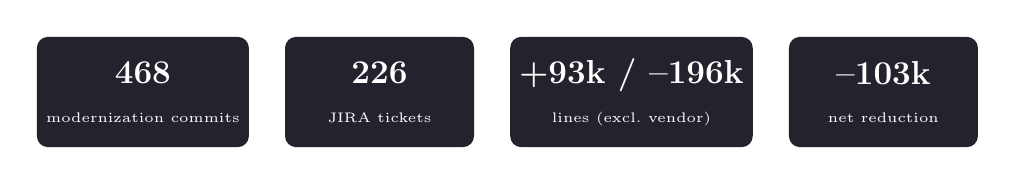
\begin{tikzpicture}
    \node (a) {\statbox{468}{modernization commits}};
    \node[right=6pt of a] (b) {\statbox{226}{JIRA tickets}};
    \node[right=6pt of b] (c) {\statbox{+93k / --196k}{lines (excl.\ vendor)}};
    \node[right=6pt of c] (d) {\statbox{--103k}{net reduction}};
  \end{tikzpicture}

  \vspace{10pt}
  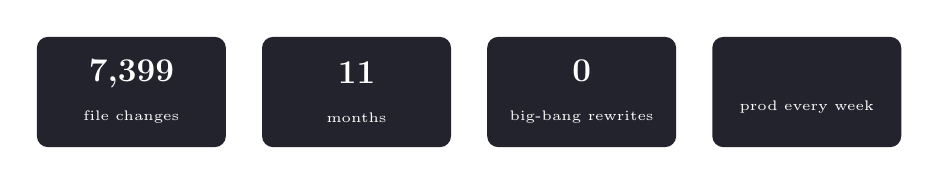
\begin{tikzpicture}
    \node (e) {\statbox{7{,}399}{file changes}};
    \node[right=6pt of e] (f) {\statbox{11}{months}};
    \node[right=6pt of f] (g) {\statbox{0}{big-bang rewrites}};
    \node[right=6pt of g] (h) {\statbox{\checkmark}{prod every week}};
  \end{tikzpicture}
\end{frame}

\begin{frame}{Commits per month}
  \centering
  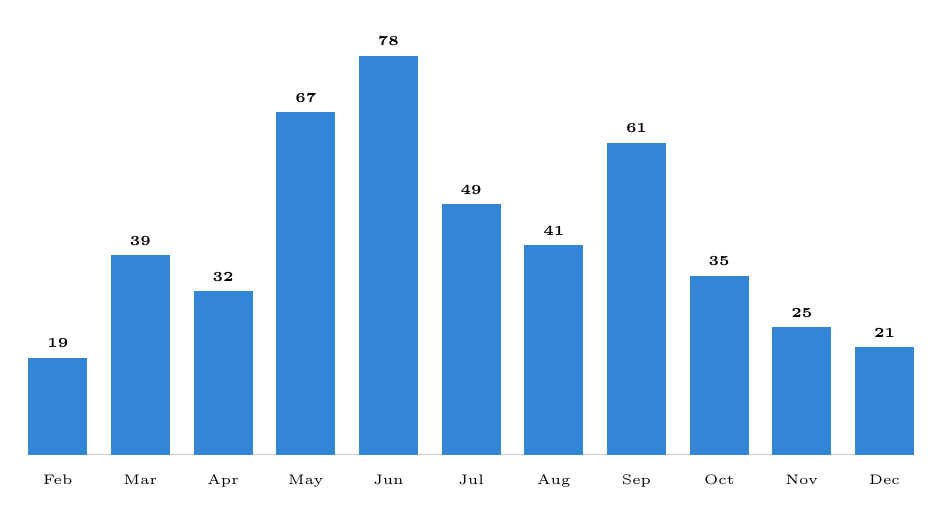
\begin{tikzpicture}[yscale=0.065, xscale=1.0]
    \draw[muted!40] (0,0) -- (11,0);
    \foreach \m/\v/\label in {0/19/Feb,1/39/Mar,2/32/Apr,3/67/May,4/78/Jun,5/49/Jul,6/41/Aug,7/61/Sep,8/35/Oct,9/25/Nov,10/21/Dec} {
      \fill[primary!80] (\m*1.05, 0) rectangle (\m*1.05+0.75, \v);
      \node[below,font=\tiny] at (\m*1.05+0.375, -2) {\label};
      \node[above,font=\tiny\bfseries] at (\m*1.05+0.375, \v) {\v};
    }
  \end{tikzpicture}
\end{frame}

% ==========================================================================
\section{Embracing the Standard Library}
% ==========================================================================

\begin{frame}{Why go back to the basics?}
  \begin{itemize}
    \setlength\itemsep{6pt}
    \item Go's \texttt{net/http} gained method-based routing in \textbf{Go 1.22}
    \item Path parameters: \texttt{r.PathValue("id")} --- no external router needed
    \item Less API surface, fewer CVEs, smaller binary
    \item The standard library is maintained by the Go team --- forever
  \end{itemize}
  \vspace{8pt}
  \alert{Principle}: \emph{``A little copying is better than a little dependency.''}
  --- Go Proverbs
\end{frame}

\begin{frame}[fragile]{Before: \texttt{go-restful} route registration}
\begin{lstlisting}
func NewBookWebService(h Handler) *restful.WebService {
	s := &restful.WebService{}
	s.Path("/books").
	  Consumes(restful.MIME_JSON).Produces(restful.MIME_JSON)

	bookID := s.PathParameter("bookID", "book ID (ISBN)").DataType("string")

	s.Route(s.POST("").Reads(entities.Book{}).To(h.Create))
	s.Route(s.PUT("/{bookID}").Param(bookID).To(h.Update))
	s.Route(s.GET("/").Param(PageSize).Param(Page).To(h.Search))
	return s
}
\end{lstlisting}
\end{frame}

\begin{frame}[fragile]{After: \texttt{net/http.ServeMux} (Go 1.22+)}
\begin{lstlisting}
func (h BookHandler) Mux() http.Handler {
	mux := http.NewServeMux()
	mux.HandleFunc("POST /books", h.Create)
	mux.HandleFunc("PUT /books/{bookID}", h.Update)
	mux.HandleFunc("GET /books", h.Search)
	mux.HandleFunc("POST /books/reviews", h.Reviews)

	sub := http.NewServeMux()
	sub.HandleFunc("GET /books/{bookID}/reviews", h.Reviews)
	mux.Handle("/books/", sub)
	return mux
}
\end{lstlisting}
\end{frame}

\begin{frame}[fragile]{Exact match with \texttt{\{$\dollar$\}}}
  Patterns without a trailing \texttt{/} already match exactly.\\
  But \texttt{GET /books/} matches all paths that have it as a prefix.

  \vspace{6pt}
\begin{lstlisting}
// matches only /books/ --- not /books/fiction, /books/42, etc.
mux.HandleFunc("GET /books/{$}", h.ListBooks)

// matches all paths with /books/ as prefix
mux.HandleFunc("GET /books/", h.CatchAll)
\end{lstlisting}

  \vspace{4pt}
  {\small Use \texttt{\{$\dollar$\}} when you need a trailing-slash route that doesn't act as a prefix.}
\end{frame}

\begin{frame}[fragile]{Working around \texttt{http.ServeMux} ambiguous pattern conflicts}
  \texttt{ServeMux} panics when patterns conflict --- e.g., \texttt{GET /books/\{bookID\}}
  and \texttt{GET /books/reviews} are ambiguous (is \texttt{reviews} a book ID?).

  \vspace{6pt}
  The fix: isolate conflicting patterns in separate muxes.

  \vspace{4pt}
\begin{lstlisting}
mux := http.NewServeMux()
mux.HandleFunc("GET /books", h.Search)
mux.HandleFunc("POST /books", h.Create)

// sub-mux for paths under /books/ avoids the conflict
sub := http.NewServeMux()
sub.HandleFunc("GET /books/{bookID}", h.GetBook)
sub.HandleFunc("GET /books/{bookID}/reviews", h.Reviews)
mux.Handle("/books/", sub)
\end{lstlisting}

  \vspace{4pt}
  {\small Strict matching catches real ambiguities, but sub-muxes let you structure routes cleanly.}
\end{frame}

\begin{frame}[fragile]{Handler signatures: before}
\begin{lstlisting}
// go-restful: library-specific types everywhere
func (h Handler) Create(req *restful.Request, resp *restful.Response) {
	var s entities.Book
	req.ReadEntity(&s)               // library-specific deserialization
	id := req.PathParameter("id")    // library-specific path params
	user := req.QueryParameter("u")  // library-specific query params
	h.ServeJSON(resp.ResponseWriter, http.StatusCreated, result)
}
\end{lstlisting}
\end{frame}

\begin{frame}[fragile]{Handler signatures: after}
\begin{lstlisting}
// net/http: only stdlib types
func (h Handler) Create(w http.ResponseWriter, r *http.Request) {
	var s entities.Book
	json.NewDecoder(r.Body).Decode(&s)  // stdlib json
	id := r.PathValue("id")             // Go 1.22+ path params
	user := r.URL.Query().Get("u")      // stdlib query params
	h.ServeJSON(w, http.StatusCreated, result)
}
\end{lstlisting}

  \vspace{6pt}
  \begin{center}
  \small
  \begin{tabular}{lll}
    \textbf{Aspect} & \textbf{go-restful} & \textbf{net/http} \\
    \hline
    Path params & \texttt{req.PathParameter()} & \texttt{r.PathValue()} \\
    Query params & \texttt{req.QueryParameter()} & \texttt{r.URL.Query().Get()} \\
    Body & \texttt{req.ReadEntity(\&v)} & \texttt{json.NewDecoder().Decode(\&v)} \\
    Response & \texttt{resp.ResponseWriter} & \texttt{w} \\
  \end{tabular}
  \end{center}
\end{frame}

% ==========================================================================
\section{Managing Third-Party Dependencies}
% ==========================================================================

\begin{frame}{45 \(\rightarrow\) 25 direct modules on \texttt{go.mod}}
  \begin{itemize}\scriptsize\setlength\itemsep{1pt}
    \item[] \added{github.com/henvic/httpretty}
    \item[] \added{github.com/henvic/pgtools}
    \item[] \added{github.com/jackc/pgerrcode}
    \item[] \added{github.com/jackc/tern/v2}
    \item[] \added{github.com/kelseyhightower/envconfig}
    \item[] \added{go.opentelemetry.io/otel}
    \item[] \removed{github.com/dgrijalva/jwt-go}
    \item[] \removed{github.com/emicklei/go-restful}
    \item[] \removed{github.com/go-openapi/\ldots}
    \item[] \removed{github.com/golang-migrate/migrate/v4}
    \item[] \removed{github.com/idebruijn/bddl}
    \item[] \removed{github.com/jessevdk/go-flags}
    \item[] \removed{github.com/lib/pq}
    \item[] \removed{github.com/pascaldekloe/goe}
    \item[] \removed{github.com/robfig/cron/v3}
    \item[] \removed{github.com/syllabix/swagserver}
    \item[] \removed{github.com/uber-go/tally/v4}
    \item[] \texttt{\ldots}
  \end{itemize}
\end{frame}

\begin{frame}{PostgreSQL}
  \begin{itemize}
    \setlength\itemsep{6pt}
    \item Previously using the \textbf{textual protocol}: values serialized as strings,
          parsed back on every query --- slow and error-prone
    \item Switched to \texttt{pgx} which uses PostgreSQL's \textbf{binary wire format} by default
    \item Native encoding of data types --- \texttt{arrays}, \texttt{jsonb}, \texttt{uuid}, \texttt{numeric} ---
          no text conversion overhead
    \item Pure SQL queries over ORMs --- we've always done this;
          full control over what runs against the database
  \end{itemize}

  \vspace{6pt}
  {\small Especially valuable for financial data where parsing precision matters.}
\end{frame}

\begin{frame}{Leveraging new Go release features}
  \begin{itemize}
    \setlength\itemsep{6pt}
    \item \textbf{Go 1.22}: method-based routing in \texttt{http.ServeMux}
    \item \textbf{Go 1.24}: \texttt{go tool} directives --- tools in \texttt{go.mod}, no \texttt{go install}
    \item \textbf{Go 1.25}: \texttt{t.Context()}
    \item \textbf{Go 1.26}: better \texttt{new(expr)}, \texttt{errors.AsType}, \texttt{slog.NewMultiHandler}, \texttt{signal.NotifyContext} now indicates which signal was received, \texttt{encoding/json/v2} (experimental), etc.
  \end{itemize}
\end{frame}

% ==========================================================================
\section{Eliminating Package-Level Globals}
% ==========================================================================

\begin{frame}{The globals problem}
  \begin{itemize}
    \setlength\itemsep{5pt}
    \item Package-level \texttt{var} for loggers, stores, metrics, validators
    \item Implicit coupling, anything can read/write them
    \item Tests must save/restore globals (\texttt{t.Cleanup} and \texttt{defer} gymnastics)
    \item Data races when tests run with \texttt{-race}
    \item Impossible to test in parallel with \texttt{-parallel} and issues with \texttt{-count}
  \end{itemize}

  \vspace{6pt}
  \textbf{Result}: correctness + made testing much easier/faster.
\end{frame}

\begin{frame}[fragile]{Before: global store}
\begin{lstlisting}
var DefaultBookStore BookStore

func copiesSold(ctx context.Context, bookID int64, since time.Time) (int, error) {
	// ...
	return DefaultBookStore.CountSales(ctx, bookID, since)
}

// app.go --- wiring via global assignment
func (app *Application) setupStore() {
	book.DefaultBookStore = app.store.book
}
\end{lstlisting}
\end{frame}

\begin{frame}[fragile]{After: struct field + constructor injection}
\begin{lstlisting}
type Service struct {
	store BookStore
	log   *slog.Logger
}

func NewService(store BookStore, log *slog.Logger) *Service {
	return &Service{store: store, log: log}
}

func (s *Service) copiesSold(ctx context.Context, bookID int64, since time.Time) (int, error) {
	// ...
	return s.store.CountSales(ctx, bookID, since)
}
\end{lstlisting}
  \vspace{4pt}
  {\small No \texttt{Init()}, no global assignment, no \texttt{t.Cleanup} restore in tests.}
\end{frame}

\begin{frame}[fragile]{Before: global logger with \texttt{Init()}}
\begin{lstlisting}
// bookmarks/package.go
var (
	log     = slog.Default()
	Metrics = metrics.NewDummy()
)
func Init(cfg config.Config) {
	log = slog.With("package", "bookmarks")  // mutation at runtime
}

func (b *Bookmarks) Save(ctx context.Context, remarks []*Remarks) {
	for _, r := range remarks {
		if err := b.save(ctx, r.ID, r.Note); err != nil {
			Metrics.Seen("bookmarks.remarks.fail", 1)  // global
			log.Error("...")                              // global
		}
	}
}
\end{lstlisting}
\end{frame}

\begin{frame}[fragile]{After: injected logger and metrics}
\begin{lstlisting}
type Bookmarks struct {
	booksRepo	booksRepo
	metrics		types.Metrics	// injected
	log		*slog.Logger	// injected
}

func NewBookmarks(repo booksRepo, m types.Metrics, log *slog.Logger) *Bookmarks {
	return &Bookmarks{
		booksRepo:	repo,
		metrics:	m,
		log:		log.With(slog.String("package", "bookmarks")),
	}
}

func (b *Bookmarks) Save(ctx context.Context, remarks []*Remarks) {
	for _, r := range remarks {
		if err := b.save(ctx, r.ID, r.Note); err != nil {
			b.metrics.Seen("bookmarks.remarks.fail", 1)    // explicit
			b.log.Error("...")                             // explicit
		}
	}
}
\end{lstlisting}
\end{frame}

\begin{frame}{The recipe ($\times$\ n)}
  \begin{enumerate}
    \setlength\itemsep{6pt}
    \item Identify the global: \texttt{var DefaultX = \ldots}
    \item Add a field to the struct that uses it
    \item No constructor? Add a new constructor
    \item Add a new constructor parameter
    \item Replace all \texttt{GlobalX.Method()} with \texttt{s.x.Method()}
    \item Delete the global and the \texttt{Init()} function
    \item Update the \texttt{app} wiring to pass the dependency
    \item \texttt{go vet ./...}, \texttt{go test -race ./...}, and \texttt{staticcheck ./...}
  \end{enumerate}

  \vspace{6pt}
  Each step is a \emph{single, reviewable commit} that ships to production.
\end{frame}

% ==========================================================================
\section{Fixing Data Races \& Parallel Testing}
% ==========================================================================

\begin{frame}{Strategy: the race detector as a refactoring guide}
  \begin{enumerate}
    \setlength\itemsep{6pt}
    \item Add \texttt{t.Parallel()} to tests "one-by-one"
    \item Run \texttt{go test -race} --- watch it light up
    \item Fix each race
    \item Revert \texttt{t.Parallel()} only where truly unsafe
    \item Eventually, add \texttt{-race} and then \texttt{-shuffle} to CI
  \end{enumerate}
\end{frame}

\begin{frame}[fragile]{Race \#1: mocked time closure}
  \textbf{Risk}: closure (that doesn't need it) captures mutex-protected state.

\begin{lstlisting}
// Before (race: f() called under RLock, but f accesses shared state)
func (r *Runner) async(f func(timeout time.Duration)) {
	r.m.RLock()
	timeout := r.getTimeout()
	defer r.m.RUnlock()
	if r.f != nil {
		return f(r.timeout)     // called while holding read lock
	}
	return nil
}
\end{lstlisting}
\begin{lstlisting}
// After
func (r *Runner) async() {
	r.m.RLock()
	timeout := r.getTimeout()           // capture reference
	r.m.RUnlock()
	if f != nil {
		return f(timeout)               // call without lock
	}
	return nil
}
\end{lstlisting}
\end{frame}

\begin{frame}[fragile]{Race \#2: slice append reallocation}
  \textbf{Problem}: \texttt{append()} can reallocate the backing array.

\begin{lstlisting}
// Before (race: append may reallocate backing array)
func TimeWhenFieldChanged(details *BookDetails, fn fieldCheck) *time.Time {
	history := append(details.History, details)
	for _, v := range history {
		if fn(v) { return &v.LastModified }
	}
	return nil
}
\end{lstlisting}
\begin{lstlisting}
// After (no allocation, no race)
func TimeWhenFieldChanged(details *BookDetails, fn fieldCheck) *time.Time {
	for _, v := range details.History {
		if fn(v) { return &v.LastModified }
	}
	if fn(details) { return &details.LastModified }
	return nil
}
\end{lstlisting}
\vspace{6pt}
  Use \texttt{go vet ./...} and \texttt{staticcheck ./...} to help you spot such problems.
\end{frame}

\begin{frame}[fragile]{Race \#3: concurrent callbacks}
\begin{lstlisting}
// Before (race: multiple callbacks append concurrently)
messages := make([]Message, 0)
notifications.Handler(func(ctx context.Context, msg Message) {
	// ...
	messages = append(messages, parsed)   // RACE
})
\end{lstlisting}
\begin{lstlisting}
// After (protected with mutex)
var (
	messages []Message
	mu       sync.Mutex
)
notifications.Handler(func(ctx context.Context, msg Message) {
	// ...
	mu.Lock()
	messages = append(messages, parsed)
	mu.Unlock()
})
\end{lstlisting}
\end{frame}

\begin{frame}{Continuous Integration enforcement}
  Add to your CI workflows:
  \begin{itemize}
    \setlength\itemsep{5pt}
    \item \texttt{go test -race ./internal/...} on unit tests
    \item \texttt{go test -shuffle on -race ./integrationtests}
    \item \texttt{go vet ./...} and \texttt{staticcheck ./...}
    \item \texttt{govulncheck ./...} for known vulnerabilities
  \end{itemize}

  \vspace{6pt}
  \alert{Any new race condition now fails the pipeline.}
\end{frame}

\begin{frame}[fragile]{Integration tests made refactoring possible}
  Mocks wouldn't catch the bugs we introduced while moving code around.\\
  Integration tests against a real PostgreSQL instance did.

  \vspace{6pt}
\begin{lstlisting}
//go:embed migrations/*.sql
var migrations embed.FS

func TestBookmarkStore(t *testing.T) {
	t.Parallel()
	conn := sqltest.Quick(t, migrations) // temp DB + migrations
	store := postgres.NewBookmarkStore(conn)

	_, err := store.Add(t.Context(), "book-1", Bookmark{
		Page: 42, Note: "important passage",
	})
	if err != nil {
		t.Fatalf("unexpected error: %v", err)
	}
}
\end{lstlisting}

  \vspace{4pt}
  {\small \texttt{sqltest.Quick} creates a temporary database, runs migrations, and cleans up --- one line of setup.}
\end{frame}

\begin{frame}{Mocks and spies still have their place}
  \begin{itemize}
    \setlength\itemsep{6pt}
    \item Integration tests verify the \emph{happy path} against real infrastructure
    \item Mocks/fakes are still valuable to simulate \textbf{failure scenarios}:
      database timeouts, connection errors, constraint violations
    \item \textbf{Spies} (see \texttt{/gen:spy}) wrap the real implementation ---
      delegate to the database by default, override individual methods when needed
    \item This gives you the best of both worlds:
      real behavior in most tests, controlled failures where it matters
  \end{itemize}
\end{frame}

\begin{frame}{End-to-end integration tests}
  The \texttt{integrationtests/} package tests the full application over HTTP.

  \vspace{6pt}
  \begin{itemize}
    \setlength\itemsep{6pt}
    \item \textbf{Dual mode}: probes a Unix socket to detect a running instance;
          if none is found, starts the entire app \emph{in-process} (ephemeral mode)
    \item \textbf{Strictly local}: multiple checks in \texttt{TestMain} enforce that tests
          only run against local development databases --- never production or staging
    \item \textbf{Self-contained}: each test gets a clean state automatically;
          helper functions let tests read like high-level scenarios
    \item \textbf{Same binary}: tests exercise the real application code, HTTP routing,
          middleware, and database queries --- not a simplified mock version
  \end{itemize}
\end{frame}

\begin{frame}[fragile]{Comparing structs with \texttt{google/go-cmp}}
\begin{lstlisting}
var dog = Animal{Name: "Dog", Class: "Mammal", Sound: "Bark"}

func TestAnimals(t *testing.T) {
	got := fetchAnimal(t.Context(), "dog")
	if diff := cmp.Diff(dog, got); diff != "" {
		t.Errorf("animal mismatch (-want +got):\n%s", diff)
	}
}
\end{lstlisting}

  \vspace{4pt}
  When a field doesn't match, you get a readable diff:

\begin{lstlisting}
  Animal{
      Name:  "Dog",
-     Class: "Mammal",
+     Class: "Reptile",
      Sound: "Bark",
  }
\end{lstlisting}

  \vspace{4pt}
  {\small When tests fail, you immediately see \emph{which} field is wrong and \emph{how}.}
\end{frame}

\begin{frame}[fragile]{Test output}
\begin{lstlisting}[language={},keywordstyle=,ndkeywordstyle=,stringstyle=,commentstyle=]
$ go test
--- FAIL: TestAnimals (0.00s)
    code_test.go:29:
            Error Trace:    animalia_test.go:29
            Error:          Not equal:
                            expected: animalia.Animal{Name:"Dog",
                              Class:"Mammal", Sound:[]string{"Bark"}}
                            actual  : animalia.Animal{Name:"Gecko",
                              Class:"Reptile", Sound:[]string{"Click"}}

                            Diff:
                            --- Expected
                            +++ Actual
                            @@ -1,6 +1,6 @@
                             (animalia.Animal) {
                            - Name: (string) (len=3) "Dog",
                            - Class: (string) (len=6) "Mammal",
                            + Name: (string) (len=5) "Gecko",
                            + Class: (string) (len=7) "Reptile",
                              Sound: ([]string) (len=1) {
                            -  (string) (len=4) "Bark"
                            +  (string) (len=5) "Click"
                              }
            Test:           TestAnimals
FAIL
exit status 1
\end{lstlisting}
  \vspace{2pt}
  {\small Source: \href{https://henvic.dev/posts/testing-go/}{\texttt{henvic.dev/posts/testing-go}}}
\end{frame}

% ==========================================================================
\section{Improving Error Handling}
% ==========================================================================

\begin{frame}{Common problems with error handling}
  \begin{enumerate}
    \setlength\itemsep{6pt}
    \item \textbf{Swallowed errors}: DB functions logging errors but returning \texttt{err = nil}
    \item \textbf{Lost error chains}: \texttt{fmt.Errorf("cannot read: \%s", err)}\\
          Fix: \texttt{fmt.Errorf("cannot read: \%w", err)}
    \item \textbf{Generic 500s}: upstream HTTP errors all become ``Internal Server Error'' or worse.
    \item \textbf{Leaking errors}: internal details exposed to clients --- security risk.
    \item \textbf{Not tracking errors}: no trace IDs, no way for users to report specific failures.
  \end{enumerate}
\end{frame}

\begin{frame}[fragile]{Fix \#1: errors that carry HTTP status codes}
\begin{lstlisting}
// types/error.go --- errors carry their intended HTTP status
type errorCode struct {
	statusCode int
	err        error
}
func (e errorCode) StatusCode() int { return e.statusCode }
func (e errorCode) Unwrap() error   { return e.err }

func Error(code int, err error) error {
	return errorCode{statusCode: code, err: err}
}

// Usage: errors declare their HTTP intent at definition
var ErrNotFound = types.Error(http.StatusNotFound, errors.New("query returned no results"))
var ErrNoPermission = types.Error(http.StatusForbidden, errors.New("insufficient permissions"))
\end{lstlisting}
\alert{Unrecognized error? Use a generic Internal Server Error.}
\end{frame}

\begin{frame}[fragile]{Fix \#2: RFC 7807 Problem Details}
\begin{lstlisting}
func (h Handler) Error(w http.ResponseWriter, r *http.Request, err error) {
	code := getStatusCode(err)       // walks Unwrap() chain
	if code == http.StatusInternalServerError {
		h.InternalServerError(w, r, "", err)
		return
	}
	problem := &api.ProblemDetails{
		Type:   "/problems/" + slugify(http.StatusText(code)),
		Title:  http.StatusText(code),
		Status: code,
		Detail: err.Error(),
	}
	Problem(w, problem)
}
\end{lstlisting}
  \vspace{2pt}
  {\small Clients get structured JSON errors with a type URI, not a plain string.}
\end{frame}

\begin{frame}[fragile]{RFC 7807 in practice}
\begin{lstlisting}
type ProblemDetails struct {
	Type       string         // URI identifying the problem type
	Title      string         // short summary (stable across occurrences)
	Status     int            // HTTP status code
	Detail     string         // human-readable, specific to this occurrence
	Instance   string         // URI for this specific occurrence
	Violations []Violation    // optional: which fields failed validation
}
\end{lstlisting}

  \vspace{4pt}
  Example response (\texttt{application/problem+json}):
\begin{lstlisting}
{
    "type":   "https://example.com/problems/not-found",
    "title":  "Not Found",
    "status": 404,
    "detail": "query returned no results"
}
\end{lstlisting}
\end{frame}

\begin{frame}[fragile]{Fix \#3: stop swallowing database errors}
\begin{lstlisting}
// Before --- error logged and silently discarded
func (s BookStore) LookupByIDs(ctx context.Context, ids []string) map[ProductDir]*Book {
	rows, err := s.db.Query(ctx, query, ids)
	if err != nil {
		slog.Error("error during LookupByIDs")   // swallowed!
	}
	return byProdCat   // may be nil or partial
}
\end{lstlisting}
\begin{lstlisting}
// After --- error returned to caller
func (s BookStore) LookupByIDs(ctx context.Context, ids []string) (map[ProductDir]*Book, error) {
	rows, err := s.db.Query(ctx, query, ids)
	if err != nil {
		return nil, fmt.Errorf("BookStore.LookupByIDs: %w", err)
	}
	return byProdCat, nil
}
\end{lstlisting}
\end{frame}

% ==========================================================================
\section{Streamlining AI in the Workflow}
% ==========================================================================

\begin{frame}{AI as a code-quality amplifier}
  \begin{itemize}
    \setlength\itemsep{6pt}
    \item \textbf{Not}: ``write my code for me''
    \item \textbf{Instead}: ``a force multiplier to take my architecture further''
  \end{itemize}

  \vspace{8pt}
  Create custom Claude skills or Gemini CLI commands. Like:
  \begin{itemize}
    \setlength\itemsep{4pt}
    \item \texttt{/gen:api} --- update Swagger/OpenAPI annotations across handlers
    \item \texttt{/gen:spy} --- generate test spy implementations for interfaces
  \end{itemize}
\end{frame}

\begin{frame}{AGENTS.md --- project conventions}
  The AI reads project rules before generating code:
  \begin{itemize}
    \setlength\itemsep{4pt}
    \item No new Go modules without explicit approval
    \item Use \texttt{go vet}, \texttt{staticcheck}, don't bother with linters
    \item No testify --- use standard \texttt{testing} + \texttt{google/go-cmp}
    \item Integration tests preferred over unit tests + mocks
    \item Use \texttt{http.ServeMux}, not routing libraries
    \item Metrics naming convention enforced
    \item \emph{``Clear is better than clever''} --- Go proverb
  \end{itemize}

  \vspace{6pt}
  \alert{The AI should follow the same code review standards as the team.}
\end{frame}

\begin{frame}[fragile]{/gen:spy --- generated test spy pattern}
\begin{lstlisting}
// Package spy is maintained using Gemini CLI with /gen:spy
// DO NOT EDIT MANUALLY UNLESS YOU MUST.

type BookmarkStore struct {
	DB                    postgres.BookmarkStore
	FindByAuthorFunc    func(ctx context.Context, author string) (Remark, error)
	findByAuthorCounter atomic.Uint32
}

func (s *BookmarkStore) FindByAuthor(ctx context.Context, author string) (Remark, error) {
	s.findByAuthorCounter.Add(1)
	if s.FindByAuthorFunc != nil {
		return s.FindByAuthorFunc(ctx, author)  // custom mock
	}
	return s.DB.FindByAuthor(ctx, author)        // real impl fallback
}
\end{lstlisting}
\end{frame}

\begin{frame}{/gen:api --- unified OpenAPI from two specs}
  \textbf{Before}: two separate \texttt{.spec} files, divergent styles, manual upkeep.
  \textbf{After}:

  \vspace{6pt}
  \begin{itemize}
    \setlength\itemsep{4pt}
    \item Merged two OpenAPI specs into one using annotations with (\href{https://github.com/swaggo/swag}{\texttt{swaggo/swag}})
    \item Changed a handler? Ask the AI to update the annotations to match
    \item Consistent response schemas, error formats, and naming across all endpoints
  \end{itemize}

  \vspace{6pt}
  \alert{One source of truth}: the code \emph{is} the API documentation.
\end{frame}

\begin{frame}[fragile]{/gen:api --- the command definition}
  \texttt{.gemini/commands/gen/api.toml}:

  \vspace{4pt}
\begin{lstlisting}[language={},keywordstyle=,ndkeywordstyle=,commentstyle=]
description = "Update API annotations and generate API docs"
prompt = """
You are an expert Go developer specialized in API documentation.
Your task is to update the Swagger/OpenAPI documentation for our REST API.
The documentation is generated from annotations in the Go source code using 'swag'.

When you identify changes in REST API endpoint handlers,
you must update the corresponding 'swag' annotations.
Ensure your annotations follow the 'swag' specification precisely.
Pay attention to things like:
- `@Summary`, `@Description`, `@Param`, `@Success`, `@Failure`, `@Router`.
- Correctly defining request and response structures.
- Data types and formats.

The user will provide the files that have changed.
Your focus should be on the files provided in `{{args}}`.
If no arguments are provided, focus on the package `internal/entrypoints/rest`.

After updating the annotations, run `make api` to regenerate the OpenAPI specification and documentation.

Do not perform any other code changes.
"""
\end{lstlisting}
\end{frame}

\begin{frame}[fragile]{Claude Code equivalent: a skill}
  \texttt{.claude/commands/gen-api.md}:

  \vspace{4pt}
\begin{lstlisting}[language={},keywordstyle=,ndkeywordstyle=,commentstyle=]
Update the Swagger/OpenAPI annotations for our REST API.
The documentation is generated from annotations in Go source
code using 'swag'.

When you identify changes in REST API endpoint handlers,
update the corresponding 'swag' annotations.
Pay attention to @Summary, @Description, @Param, @Success,
@Failure, @Router.

Focus on the files provided in $ARGUMENTS.
If no arguments are provided, focus on
`internal/entrypoints/rest`.

After updating the annotations, run `make api`.

Do not perform any other code changes.
\end{lstlisting}

  \vspace{4pt}
  {\small Invoke with \texttt{/gen-api} or \texttt{/gen-api internal/entrypoints/rest}}
\end{frame}

\begin{frame}[fragile]{/gen:api --- annotated handler example}
\begin{lstlisting}
// AddBookmark godoc
// @Summary      Add a bookmark to a book
// @Tags         bookmarks
// @Accept       json
// @Produce      json
// @Param        bookID path string true "Book ID"
// @Param        body body AddBookmarkRequest true "Bookmark"
// @Success      201 {object} Bookmark
// @Failure      400 {object} api.ProblemDetails
// @Failure      404 {object} api.ProblemDetails
// @Router       /bookmarks/{bookID} [post]
func (h Handler) AddBookmark(w http.ResponseWriter, r *http.Request) {
	bookID := r.PathValue("bookID")
	var req AddBookmarkRequest
	if err := json.NewDecoder(r.Body).Decode(&req); err != nil {
		h.Error(w, r, types.Error(http.StatusBadRequest, err))
		return
	}
	bookmark, err := h.service.Add(r.Context(), bookID, req)
	if err != nil {
		h.Error(w, r, err)
		return
	}
	h.ServeJSON(w, http.StatusCreated, bookmark)
}
\end{lstlisting}
\end{frame}

\begin{frame}[fragile]{Step 1: you change the code}
  Add two fields to the request struct:

\begin{lstlisting}
type AddBookmarkRequest struct {
	Page    int      `json:"page"`
	Note    string   `json:"note"`
	Section string   `json:"section"`  // new
	Tags    []string `json:"tags"`     // new
}
\end{lstlisting}

  \vspace{4pt}
  Then run \texttt{/gen:api} --- the AI reads the code and updates the annotations.
\end{frame}

\begin{frame}[fragile]{Step 2: AI updates the annotations}
\begin{lstlisting}
  // AddBookmark godoc
  // @Summary      Add a bookmark to a book
\end{lstlisting}
\begin{lstlisting}[commentstyle=\itshape\color{added}]
+ // @Description  Creates a bookmark with optional section and tags
\end{lstlisting}
\begin{lstlisting}
  // @Tags         bookmarks
  // @Accept       json
  // @Produce      json
  // @Param        bookID path string true "Book ID"
  // @Param        body body AddBookmarkRequest true "Bookmark"
  // @Success      201 {object} Bookmark
  // @Failure      400 {object} api.ProblemDetails
  // @Failure      404 {object} api.ProblemDetails
  // @Router       /bookmarks/{bookID} [post]
\end{lstlisting}

  \vspace{4pt}
  {\small Barely no manual doc maintenance. Change the code \(\rightarrow\) let the AI catch up.}
\end{frame}

% ==========================================================================
\section{Project Structure \& Other Improvements}
% ==========================================================================

\begin{frame}{Restructuring project layout}
  \begin{columns}[T]
    \begin{column}{0.42\textwidth}
      \textbf{Before}\vspace{2pt}
      \begin{itemize}\scriptsize\setlength\itemsep{1pt}
        \item \texttt{cmd/bookstore/main.go}
        \item \texttt{cmd/bookstore/config.go}
        \item \texttt{pkg/bookstore/bookmarks/}
        \item REST endpoints in multiple packages
        \item Cronjobs scheduled on services + database
      \end{itemize}
    \end{column}
    \begin{column}{0.54\textwidth}
      \textbf{After}\vspace{2pt}
      \begin{itemize}\scriptsize\setlength\itemsep{1pt}
        \item \texttt{main.go} (root level)
        \item \texttt{internal/app/}
        \item \texttt{internal/config/}
        \item \texttt{internal/bookcollection/}
        \item \texttt{internal/entrypoints/rest/}
        \item \texttt{internal/entrypoints/cronjobs/}
        \item \texttt{internal/entrypoints/subscription/}
        \item Cronjobs using Kubernetes
      \end{itemize}
    \end{column}
  \end{columns}

  \vspace{4pt}
  \centering
  {\small Clear separation: entrypoints \(\rightarrow\) business logic \(\rightarrow\) entities}\\[2pt]
  {\small Domain types extracted into a shared \texttt{internal/entities/} layer to mitigate circular dependency hacks}
\end{frame}

\begin{frame}{Improvements shipped incrementally}
  \begin{itemize}
    \setlength\itemsep{2pt}
    \item \textbf{Metrics}: replaced \texttt{uber-go/tally} with Prometheus library
    \item \textbf{Cronjobs}: in-app scheduling \(\rightarrow\) Kubernetes CronJobs
    \item \textbf{Tracing}: OpenTelemetry on HTTP clients and servers
    \item \textbf{Context}: fixed cancellation in reading flow
    \item \textbf{Shutdown}: Unix socket-based graceful shutdown
    \item \textbf{Integration tests}: in-process infra, auto-discover address
    \item \textbf{Profiling}: \texttt{pprof} locally and in production via \href{https://docs.cloud.google.com/profiler/docs/profiling-go}{Cloud Profiler}
    \item \textbf{Observability}: Kubernetes alerts, health check endpoints
    \item \textbf{CI pipeline}: consolidated stages, faster feedback loop
    \item \textbf{PostgreSQL}: \texttt{database/sql} \(\rightarrow\) \texttt{pgx} with powerful native binary protocol
  \end{itemize}
\end{frame}

% ==========================================================================
\section{Results \& Lessons Learned}
% ==========================================================================

\begin{frame}{Results}
  \begin{itemize}
    \setlength\itemsep{5pt}
    \item \textbf{103{,}000 lines deleted} (net) --- the codebase \emph{shrank}
    \item \textbf{Zero data races} in CI (enforced by \texttt{-race} flag)
    \item \textbf{Zero greenfield rewrites} --- every commit shippable
    \item \textbf{5 major dependencies removed} --- replaced by stdlib or smaller libs
    \item \textbf{23+ package-level globals eliminated}
    \item \textbf{Structured errors} with RFC 7807 across all API endpoints
    \item \textbf{AI-maintained} API docs and test spies reduce toil
    \item \textbf{Tests run faster} and are more reliable (in parallel, no shared state)
    \item \textbf{6 contributors} participated in the modernization effort
  \end{itemize}
\end{frame}

\begin{frame}{Lessons learned}
  \begin{enumerate}
    \setlength\itemsep{6pt}
    \item \textbf{Small commits win.}
          Each change is reviewable and revertible.
    \item \textbf{The race detector is a refactoring tool.}
          Add \texttt{-race} early.
    \item \textbf{Globals are the root of all evil.}
          Dependency Injection in Go is just a struct field and a constructor parameter.
    \item \textbf{AI works best with clear rules.}
          Write your conventions down.
    \item \textbf{Good practices are contagious.}
          Once the pattern is visible in the codebase, others follow.
    \item \textbf{You don't need a rewrite.}
          You need a direction and discipline.
  \end{enumerate}
\end{frame}

\begin{frame}{Key takeaways}
  \centering
  \vspace{10pt}
  {\large
  \begin{tabular}{rl}
    \textcolor{primary}{\textbf{1.}} & Embrace the standard library \\[8pt]
    \textcolor{primary}{\textbf{2.}} & Remove globals, inject dependencies \\[8pt]
    \textcolor{primary}{\textbf{3.}} & Let \texttt{-race} guide your refactoring \\[8pt]
    \textcolor{primary}{\textbf{5.}} & Ship incremental improvements, every week \\[8pt]
    \textcolor{primary}{\textbf{6.}} & Let AI amplify good practices, not replace them \\
  \end{tabular}
  }
\end{frame}

\begin{frame}{Resources}
  \begin{itemize}
    \setlength\itemsep{8pt}
    \item \href{https://henvic.dev/posts/testing-go/}{\textbf{henvic.dev/posts/testing-go}}\\
          {\small On testing Go code using the standard library}
    \item \href{https://github.com/henvic/pgxtutorial}{\textbf{github.com/henvic/pgxtutorial}}\\
          {\small Tutorial: building a Go service with PostgreSQL and gRPC/HTTP (\href{https://henvic.dev/posts/go-postgres/}{post})}
    \item \href{https://github.com/henvic/httpretty}{\textbf{github.com/henvic/httpretty}}\\
          {\small HTTP client/transport inspector for debugging REST requests}
    \item \href{https://github.com/henvic/pgtools}{\textbf{github.com/henvic/pgtools}}\\
          {\small Helpers for PostgreSQL and Go using pgx, tern, and scany; including \href{https://pkg.go.dev/github.com/henvic/pgtools/sqltest}{pgtools/sqltest}}
    \item \href{https://github.com/henvic/pgq}{\textbf{github.com/henvic/pgq}}\\
          {\small Query builder for PostgreSQL (if you insist on using one)}
  \end{itemize}
\end{frame}

\begin{frame}[standout]
  Thank you!

  \vspace{16pt}
  {\normalsize
  Henrique Vicente de Oliveira Pinto\\[4pt]
  \href{https://henvic.dev/}{\texttt{henvic.dev}}\\[10pt]
  bol \(\times\) ING Tech Talks --- Amsterdam
  }
\end{frame}

\end{document}
